%% Based on a TeXnicCenter-Template by Gyorgy SZEIDL.
%%%%%%%%%%%%%%%%%%%%%%%%%%%%%%%%%%%%%%%%%%%%%%%%%%%%%%%%%%%%%

%------------------------------------------------------------
%
\documentclass[letterpaper,10pt]{article}%
%Options -- Point size:  10pt (default), 11pt, 12pt
%        -- Paper size:  letterpaper (default), a4paper, a5paper, b5paper
%                        legalpaper, executivepaper
%        -- Orientation  (portrait is the default)
%                        landscape
%        -- Print size:  oneside (default), twoside
%        -- Quality      final(default), draft
%        -- Title page   notitlepage, titlepage(default)
%        -- Columns      onecolumn(default), twocolumn
%        -- Equation numbering (equation numbers on the right is the default)
%                        leqno
%        -- Displayed equations (centered is the default)
%                        fleqn (equations start at the same distance from the right side)
%        -- Open bibliography style (closed is the default)
%                        openbib
% For instance the command
%           \documentclass[a4paper,12pt,leqno]{article}
% ensures that the paper size is a4, the fonts are typeset at the size 12p
% and the equation numbers are on the left side
%
\usepackage{amsmath}%
\usepackage{amsfonts}%
\usepackage{amssymb}%
\usepackage{graphicx,color}

\oddsidemargin=0.0in
\evensidemargin=0.0in
\textwidth=6.5in
\headheight=0.25in
\topmargin=0.0in
\textheight=8.5in


%-------------------------------------------
\newtheorem{theorem}{Theorem}
\newtheorem{acknowledgement}[theorem]{Acknowledgement}
\newtheorem{algorithm}[theorem]{Algorithm}
\newtheorem{axiom}[theorem]{Axiom}
\newtheorem{case}[theorem]{Case}
\newtheorem{claim}[theorem]{Claim}
\newtheorem{conclusion}[theorem]{Conclusion}
\newtheorem{condition}[theorem]{Condition}
\newtheorem{conjecture}[theorem]{Conjecture}
\newtheorem{corollary}[theorem]{Corollary}
\newtheorem{criterion}[theorem]{Criterion}
\newtheorem{definition}[theorem]{Definition}
\newtheorem{example}[theorem]{Example}
\newtheorem{exercise}[theorem]{Exercise}
\newtheorem{lemma}[theorem]{Lemma}
\newtheorem{notation}[theorem]{Notation}
\newtheorem{problem}[theorem]{Problem}
\newtheorem{proposition}[theorem]{Proposition}
\newtheorem{remark}[theorem]{Remark}
\newtheorem{solution}[theorem]{Solution}
\newtheorem{summary}[theorem]{Summary}
\newenvironment{proof}[1][Proof]{\textbf{#1.} }{\ \rule{0.5em}{0.5em}}

\begin{document}

\title{Compiling GMAT using Visual Studio 2010}
\author{Darrel J. Conway\thanks{Support provided by NASA GSFC FDSS Contract, Task 28.}
\\Thinking Systems, Inc.\\Tucson, AZ}
\date{\today}
\maketitle

\begin{abstract}
This document describes the steps needed to build GMAT using Visual Studio 2010 (VS2010).  The instructions start with a fresh installation of VS2010, provide directions for installing wxWidgets, and finally for building GMAT.
\end{abstract}

\section{Introduction}

The General Mission Analysis Tool, GMAT, is a space trajectory optimization and mission analysis system developed by NASA and private industry in the spirit of the NASA Vision. GMAT contains new technology and is a testbed for future technology development. To satisfy NASA's mandate and maximize technology transfer, GMAT is an open source software system licensed under the NASA Open Source Agreement.  Interested parties are encouraged to use GMAT to plan spacecraft missions, to build the system when they have requirements for features not yet included in GMAT, and to contribute new capabilities to the system either through direct contributions to the code base or through plugin libraries.

This document describes the steps a new developer takes to set up a build environment for GMAT using Microsoft's Visual Studio development system.  The instructions were written using Visual Studio 2010 Express Edition, and validated using both the Express Edition and the Professional Edition.  The following instructions assume that the developer is running a Windows XP, Vista, or Windows~7 based computer.  Separate instructions are available for users building GMAT with the GNU Compiler Collection (gcc) on Windows, Mac, or Linux based computers.

The following sections describe installation of the compiler, folder arrangements and code used in the GMAT build files, preliminary steps necessary to collect and build the libraries GMAT needs, and the build steps for GMAT itself.  The document concludes with instructions for plugin libraries that GMAT uses to interface with MATLAB and the MATLAB Optimization toolbox, to perform estimation (the estimation plugin is a preview of capabilities still in development), and the VF13ad optimizer (core code available separately).

\section{Installing Visual C++ / Visual Studio 2010 Express Edition}

The Visual C++ environment can be installed either from a web-based installer or from disk.  Users of the paid versions of Visual C++ should skip this section and install the product following the instructions provided by Microsoft.  Users of the Express edition can install from the online instructions provided by Microsoft, or by following the instructions provided here.

\subsection{Option 1: Web installation}

Visual C++ can be installed using a web based installer by following these steps:

\begin{enumerate}
	\item Open a web browser and browse to the Visual Studio 2010 Express download page: \\http://www.microsoft.com/express/Downloads/\#2010-Visual-CPP
	\item Download the installer for Visual C++
	\item Open the installer (vc\_web.exe) by double clicking on it
	\item Follow the installation instructions
\end{enumerate}

\subsection{Installing from a Disk Image}

If you have a disk containing Visual Studio Express, follow these steps:

\begin{figure}
\centering

\includegraphics{DiskStart.eps}
\caption{Screen for a New Disk}
\label{fig:DiskStart}
\end{figure}

\begin{figure}
	\centering
		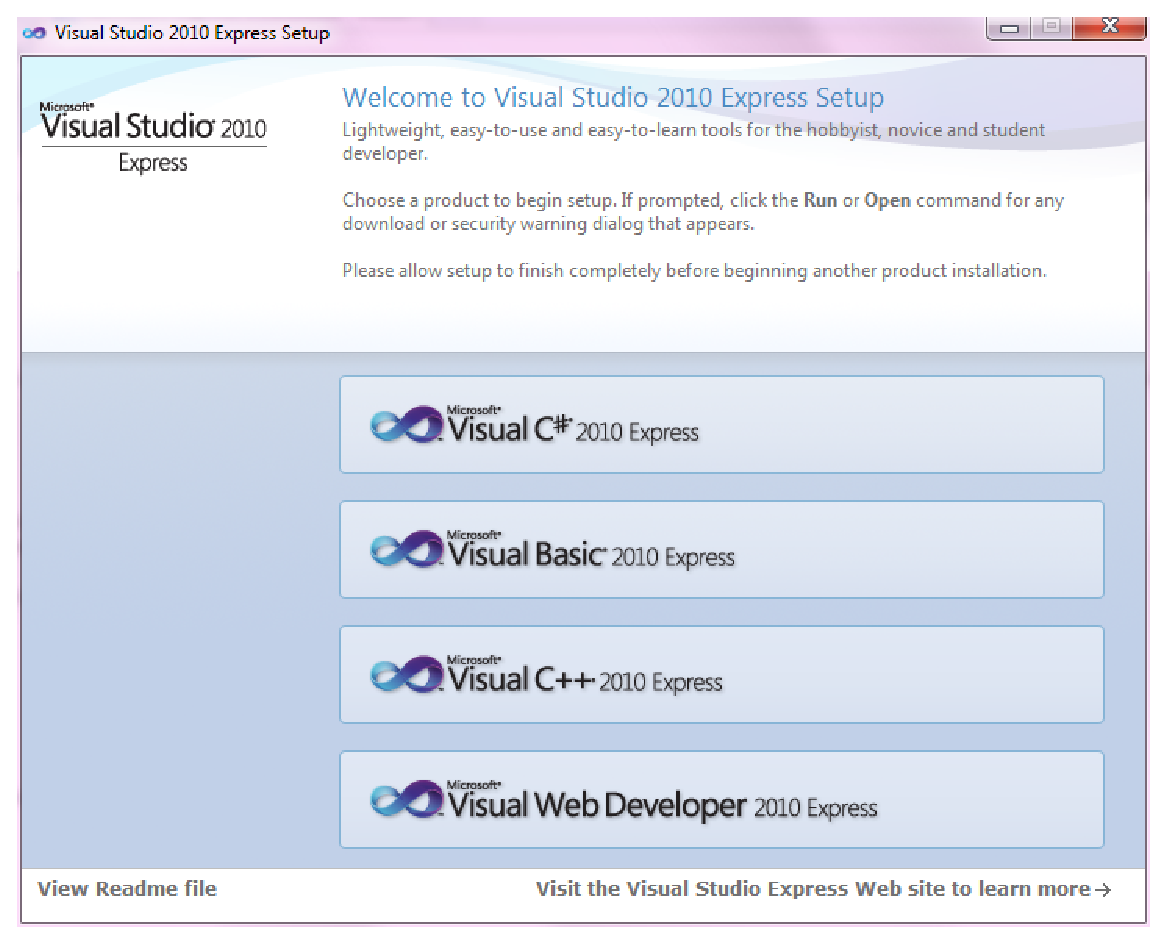
\includegraphics[scale=0.5]{VisualCpp.eps}
	\caption{Select Visual C++ Here}
	\label{fig:VisualCpp}
\end{figure}

\begin{enumerate}
\item Put the installation disk into your DVD drive
\item If prompted, select ``Run Setup.hta'' from the Autoplay Menu (See Figure~\ref{fig:DiskStart})
\item Select Visual C++ 2010 Express from the menu that opens (See Figure~\ref{fig:VisualCpp})
\item Follow the installation instructions.  GMAT does not require SQLServer, so you can deselect that option for installation.
\end{enumerate}

\subsection{64-bit Compilers (Optional)}

If you plan to build the 64-bit version of GMAT{\footnote{The GMAT development team does not maintain the 64-bit builds of the system.  Project settings and source code files for 64-bit builds are not guaranteed to work without some user interaction to correct changes that may not have been checked in 64-bit compilations.}, you'll need to install the Windows 7 SDK version 7.1.  You'll also need to be running on a 64-bit version of Windows so you can test the resulting build.

The SDK can be downloaded from (all on one line)
\begin{quote}
\begin{verbatim}
http://www.microsoft.com/downloads/en/details.aspx?FamilyID=6b6c21d2-2006-4afa-
9702-529fa782d63b\&displaylang=en
\end{verbatim}
\end{quote}
\noindent Download the web based installer by clicking on the ``Download'' button, and then run it.  This installs the software development kit, including a 64-bit compiler.

\section{Folder Configuration}

Create a folder for building GMAT.  I'll use C:\textbackslash GmatVS as the root folder in this document.  This folder will contain the subfolders for third party components of the build -- wxWidgets, cspice, pcrecpp, and similar files.  Add the following folders to your root folder:
\begin{itemize}
\item Gmat3rdParty
\item GmatDevelopment
\item GmatPlugins (if you will be using the configuration managed plugin libraries)
\end{itemize}

\noindent Inside of the Gmat3rdParty folder, create the following subfolders; for the 32-bit builds:
\begin{itemize}
\item cspice
\item f2c
\item pcre
\item wxWidgets
\end{itemize}

\begin{figure}
\centering
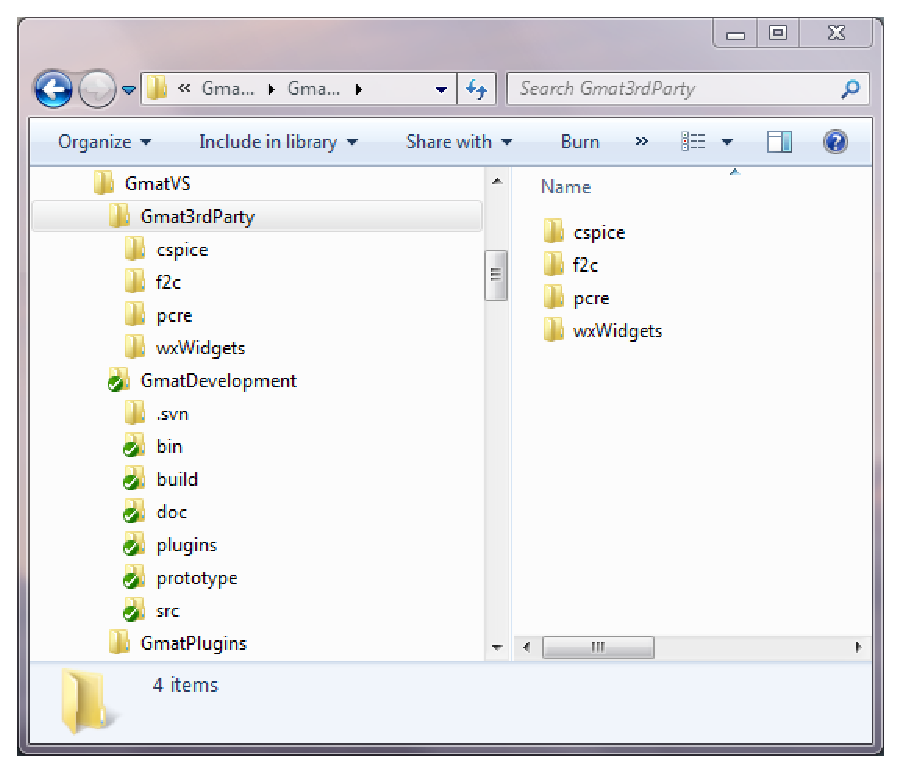
\includegraphics[scale=0.75]{FolderStructure.eps}
\caption{The File Structure used in GMAT's Configuration Managed Build Files}
\label{fig:FolderStructure}
\end{figure}


\noindent At this point, your folder structure should match the structure shown in Figure~\ref{fig:FolderStructure}.  If you want to also build the 64-bit release and have either a paid version of Visual Studio 2010 (that is, Professional, Premium, or Ultimate), or if you installed the 64-bit tools in the Windows SDK, add these folders for the 64-bit versions of the 3rd party tools:
\begin{itemize}
\item cspice64
\item f2c64
\item pcre64
\item wxWidgets64
\end{itemize}

\section{Downloading GMAT}

GMAT's source code is located in a Subversion repository at SourceForge.  In addition to the source code, the repository at SourceForge contains the build files we'll need to proceed, including wxWidgets project files configured for Visual Studio 2010.  Because of this, you need to begin by downloading the GMAT development code using a Subversion client.  I am using SmartSVN on Windows, but any client should work.  Set up your client to access code at the following URL:
\begin{quote}
https://svn.code.sf.net/p/gmat/code/trunk
\end{quote}
\noindent Check out the entire source tree from that location into the GmatDevelopment folder you created earlier.  When you check out the tree, you'll retrieve GMAT's source code, development files, documentation, source for several plugin libraries, and the support files needed to run GMAT.

Alternatively, if you can access Subversion from a command prompt, you can download the code directly by setting to your current diractory to the root folder containing the GmatDevelopment and Gmat3rdParty folders and then entering the command
\begin{quote}
svn checkout svn://svn.code.sf.net/p/gmat/code/trunk GmatDevelopment
\end{quote}

\section{Building wxWidgets}

From this point through Section~\ref{sec:Plugins} we will concentrate on the 32-bit build of GMAT.  Appendix~\ref{app:64bit} describes the settings and changes necessary to build GMAT as a 64-bit application.  We begin by building wxWidgets, the GUI toolkit used for GMAT's user interface.

\subsection{Install the wx Code}

\begin{enumerate}
\item Download wxWidgets 2.8 from http://wxwidgets.org/downloads/.  Use the latest stable version of the 2.8 tree (2.8.12 at this writing), and download the wxMSW zip package.
\item Unpack the wx code into the folder named wxWidgets in your Gmat3rdParty folder.  You should see folders named art, build, contrib, demos, docs, include, lib, locale, samples, src, and utils in the wxWidgets folder when finished.
\item Visual Studio 2010 has trouble processing the Visual C++ project files that ship with wx.  Instead, we'll use files already configured for wx at Thinking Systems.
\begin{enumerate}
\item The Visual Studio 2010 solution and project files for wxWidgets are located in an archive file in the GMAT folders you checked out earlier.  Find the file wxWidgets.zip in the build\textbackslash windows-VS2010 folder of that working copy of the code.
\item Unpack the wxWidgets.zip archive into your wxWidgets folder, overwriting existing files as necessary.
\item Check to see that the file wx\_dll.sln is in your Gmat3rdParty\textbackslash wxWidgets\textbackslash build\textbackslash msw folder.  (This step ensures that all of the build files are properly positioned in the wxWidgets folder structure.  The key files are wx\_dll.sln in the Gmat3rdParty\textbackslash wxWidgets\textbackslash build\textbackslash msw folder and wxcontrib\_dll.sln in the Gmat3rdParty\textbackslash wxWidgets\textbackslash contrib\textbackslash build folder.)
\end{enumerate}

\end{enumerate}

\subsection{Prepare and Build wxWidgets}
\begin{enumerate}
\item Open Visual Studio
\item Select ``File | Open | Project/Solution...'' from the menu bar
\item Open the wx\_dll.sln solution file from the build\textbackslash msw folder of your wxWidgets installation.  (For me, the file is found in  C\:\textbackslash GmatVS\textbackslash Gmat3rdParty\textbackslash wxWidgets\textbackslash build\textbackslash msw)
\item GMAT needs the wxWidgets OpenGL components as part of the build.  This setting is configured in the wx\textbackslash setup.h configuration file for the build.  We need to change a setting in this file from its default setting.
\begin{enumerate}
	\item Open one of the projects in the Visual Studio solution tree
	\item Open the Setup Headers folder in this project
	\item Open the first setup.h file in the folder by double clicking on it
	\item If this file has the line ``\textbackslash\textbackslash  Name:        wx/univ/setup.h'' at the top, open the other setup file. (You want to edit the file in msw rather than in univ; the file you want identifies itself as ``wx/msw/setup.h''.)
	\item Search for wxUSE\_GLCANVAS in the open file
	\item Set wxUSE\_GLCANVAS to 1 rather than the default value of 0
	\item Save and close the file.
\end{enumerate}
\item On the Visual C++ toolbar select ``DLL Release'' (specifying the build configuration) and set your solution platform to Win32.  Figure~\ref{fig:wxSettings} shows these settings.
\item Build the solution (right click on the ``Solution wx\_dll{}'' node at the top of the tree and select ``Build Solution''.)
\item Most, but not all, of the solution will build.  You may need to repeat the build process to get all of the libraries GMAT requires built.  Build the solution again until all but the dbgrid projects build.  (You are done when 19 of the 20 projects build.)
\item Select ``File | Open | Project/Solution...'' from the menu bar
\item Open the wxcontrib\_dll.sln solution file from the contrib\textbackslash build folder of your wxWidgets installation.  (For me, the file is found in  C\:\textbackslash GmatVS\textbackslash Gmat3rdParty\textbackslash wxWidgets\textbackslash contrib\textbackslash build)
\item On the Visual C++ toolbar select ``DLL Release'' (specifying the build configuration) and set your solution platform to Win32.
\item Build the solution (right click on the ``Solution wxcontrib\_dll'' node at the top of the tree and select ``Build Solution''.)
\end{enumerate}

\begin{figure}
\centering
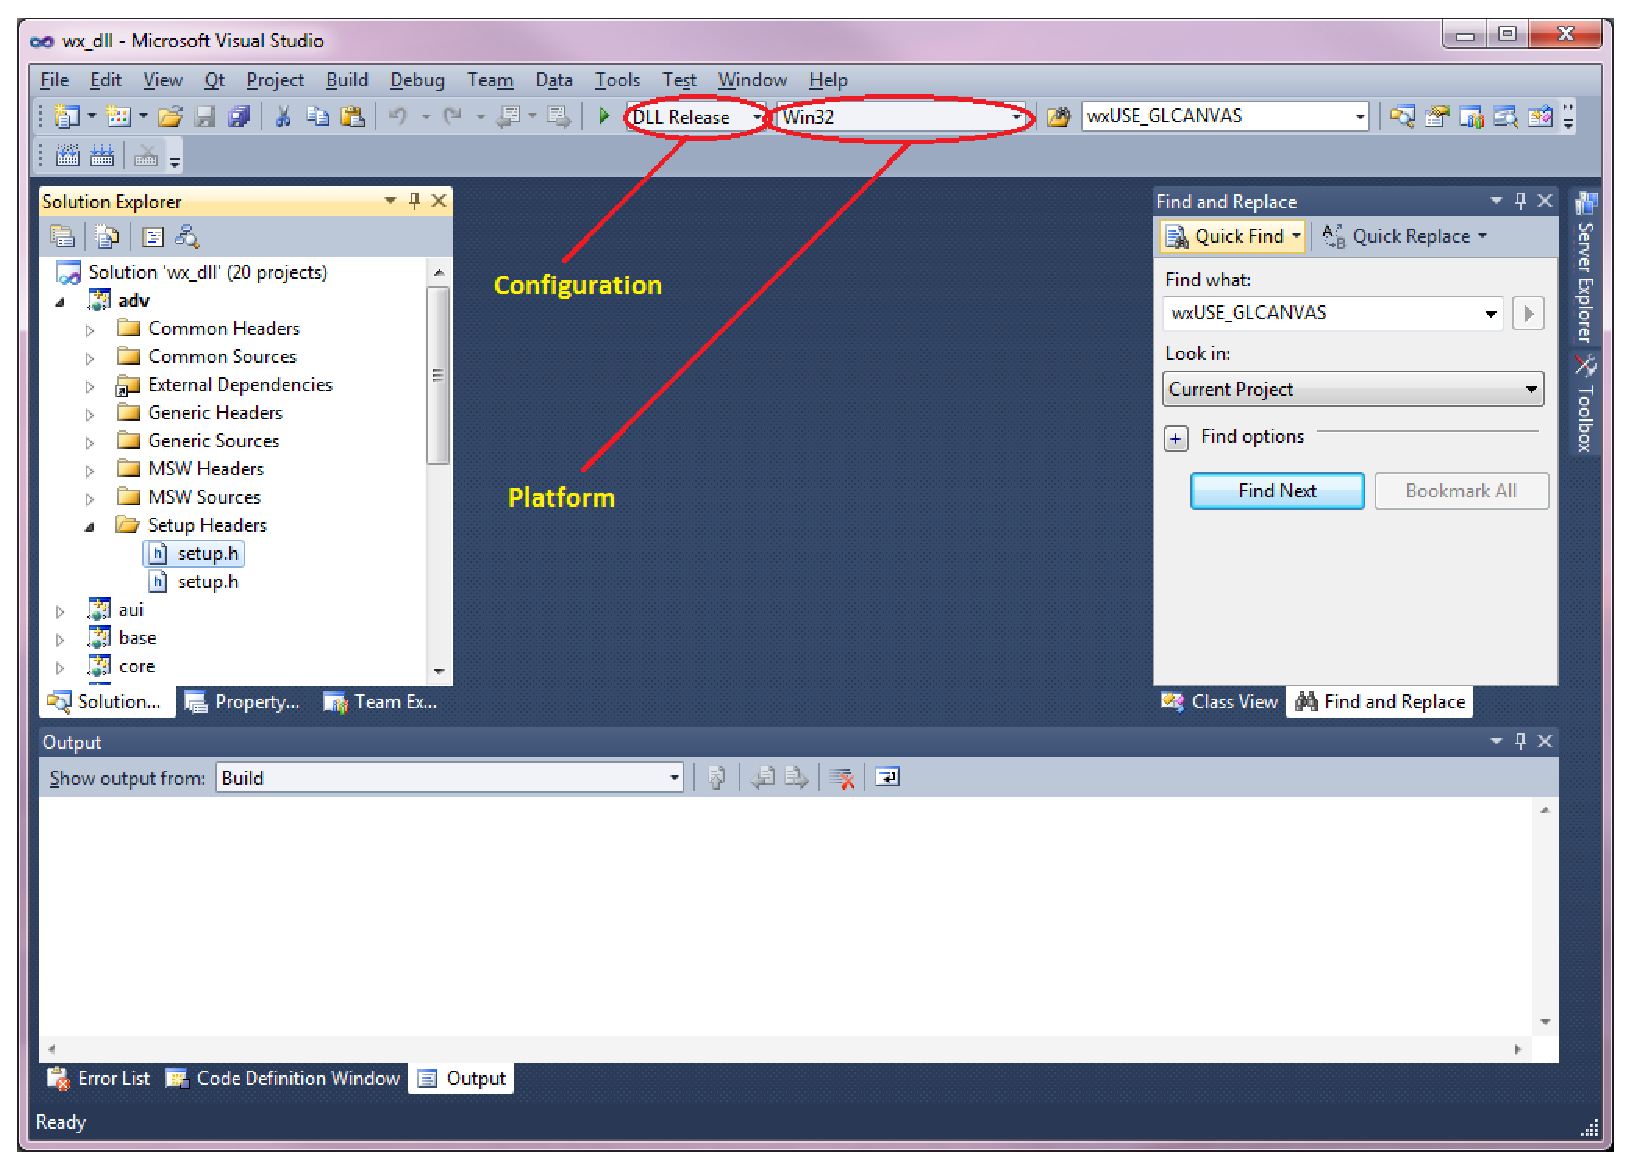
\includegraphics[scale=0.6]{DLLRelease.eps}
\caption{Configuration and Platform Settings for the 32-bit wxWidgets Build}
\label{fig:wxSettings}
\end{figure}

\noindent Check to see that you have 15 dll files in the wxWidgets\textbackslash lib\textbackslash vc\_dll folder:
{\begin{itemize}\setlength{\itemsep}{0pt}
\item wxbase28\_net\_vc\_custom.dll
\item wxbase28\_odbc\_vc\_custom.dll
\item wxbase28\_vc\_custom.dll
\item wxbase28\_xml\_vc\_custom.dll
\item wxmsw28\_adv\_vc\_custom.dll
\item wxmsw28\_aui\_vc\_custom.dll
\item wxmsw28\_core\_vc\_custom.dll
\item wxmsw28\_gl\_vc\_custom.dll
\item wxmsw28\_html\_vc\_custom.dll
\item wxmsw28\_media\_vc\_custom.dll
\item wxmsw28\_netutils\_vc\_custom.dll
\item wxmsw28\_qa\_vc\_custom.dll
\item wxmsw28\_richtext\_vc\_custom.dll
\item wxmsw28\_stc\_vc\_custom.dll
\item wxmsw28\_xrc\_vc\_custom.dll
\end{itemize}}

\noindent Copy these into your GmatDevelopment\textbackslash application\textbackslash bin folder.

\subsection{(Optional) Preparing for Debug Builds}

The GMAT solution file can be used to build a debug version of GMAT.  In order to use that version, you will need to build a set of wxWidgets debug libraries.  The procedure is the same as for the release build as described above, with the following changes:

\begin{itemize}
\item On the Visual C++ toolbar select ``DLL Debug'' rather than ``DLL Release'' as the solution configuration.
\item After building the libraries, the debug versions will all have the letter ``d'' added to the library name: wxbase28d\_net\_vc\_custom.dll, wxbase28d\_odbc\_vc\_custom.dll, etc.  Copy these files into your GmatDevelopment\textbackslash application\textbackslash debug folder.
\end{itemize}

\section{Preparing SPICE}

GMAT includes readers and writers for data in the SPICE kernel format supplied by the Jet Propulsion Laboratory (JPL).  In order to build GMAT, you'll need to add the SPICE libraries to your system.  To do this, follow these steps:

\begin{enumerate}
\item Download the SPICE toolkit for Visual C.  The 32-bit edition is available from
\begin{quote}
http://naif.jpl.nasa.gov/naif/toolkit\_C\_PC\_Windows\_VisualC\_32bit.html
\end{quote}
\noindent and the 64-bit version from
\begin{quote}
http://naif.jpl.nasa.gov/naif/toolkit\_C\_PC\_Windows\_VisualC\_64bit.html
\end{quote}
\noindent You want the file named cspice.zip.
\item Unpack the archive into your Gmat3rdParty\textbackslash cspice (or cspice64 for 64-bit) folder.  You should unpack the files so that you have, for example, a Gmat3rdParty\textbackslash cspice\textbackslash include folder that contains the cspice header (.h) files.
\end{enumerate}

\noindent Note that cspice includes Fortran to C (f2c) library code, so you do not need to manage f2c separately when working with the GMAT base library code.

\section{Building GMAT}

At this point, GMAT should build without further configuration.  Follow these steps:
\begin{enumerate}
\item Open Visual C++
\item Select ``File | Open | Project/Solution...'' from the menu bar
\item Browse to the GmatDevelopment\textbackslash build\textbackslash windows-VS2010 folder
\item Select the GmatVS2010.sln solution file and click the Open button.  The GMAT solution will open and show projects to build GMAT and several plugin libraries.
\item The solution has two configurations, depending on how you want to proceed: Debug and Release.  Select the configuration that you would like to build.
\item Right click on the top node in the Solution Explorer, and select Rebuild to completely build GMAT including all of the plugins, but excluding the console application.  This process takes a few minutes.
\item Open Windows Explorer and browse to your GmatDevelopment\textbackslash application\textbackslash bin or your GmatDevelopment\textbackslash application\textbackslash debug folder based on the configuration you selected.  You should see GMAT.exe there, along with libGmatBase.dll and your wxWidgets libraries.
\item Double click on the GMAT.exe file to run GMAT.  Press the Run button to run the default mission.  Rejoice.
\end{enumerate}

\section{Building the Plugin Libraries for MATLAB, fmincon, Estimation, and the C-Interface (Optional)}

At this writing there are four plugin libraries included in GMAT's trunk code on SourceForge.  Two of these, libMatlabInterface and libFminconOptimizer, require a recent version of MATLAB to build.  The other two, libGmatEstimation and libCInterface, build in a straightforward manner.  We'll look at the latter two first, and then at the MATLAB dependent plugins.

\subsection{Building libGmatEstimation and libCInterface}

GMAT's source tree includes a project file and code for a GMAT compatible estimation plugin.  This plugin includes both a Kalman filter and a batch estimator, along with a measurement simulator and several measurement models.  At this writing, these components are in an early alpha form.  As the component evolves, the build process should remain the same.  GMAT's estimation plugin includes tropospheric and ionospheric models.  The ionosphere model was originally coded in Fortran, and then imported into the GMAT plugin using the f2c utility program.  For that reason, you must have either f2c or SPICE installed to build the estimation plugin.

The source tree also includes code for a C interface into GMAT's object-oriented engine in the shared library libGmatBase.  The C-interface is being used on other projects to provide access to select components of GMAT's engine for external use.  This access is contained in the libCInterface plugin.

Follow these instructions to build libGmatEstimation and libCInterface:

\begin{enumerate}
\item Building libGmatEstimation
\begin{enumerate}
\item Open Visual C++
\item Select ``File | Open | Project/Solution...'' from the menu bar
\item Browse to the GmatDevelopment\textbackslash build\textbackslash GmatVS2010 folder
\item Select the GmatVS2010.sln solution file and click the Open button.  The GMAT solution will open and show projects to build GMAT and several plugin libraries.
\item Right-click on the libGmatEstimation node, and select ``Build''
\end{enumerate}
\item Building libCInterface
\begin{enumerate}
\item Open Visual C++
\item Select ``File | Open | Project/Solution...'' from the menu bar
\item Browse to the GmatDevelopment\textbackslash build\textbackslash GmatVS2010 folder
\item Select the GmatVS2010.sln solution file and click the Open button.  The GMAT solution will open and show projects to build GMAT and several plugin libraries.
\item Right-click on the libCInterface node, and select ``Build''
\end{enumerate}
\end{enumerate}

Once each build finishes, the plugin libraries will be copied to the appropriate target folders.  The release build of libGmatEstimation is copied into the application/plugins folder, and the release build of libCInterface, into the application/bin folder.

\subsection{The MATLAB and fmincon Plugins}

Next we will build the GMAT MATLAB interface.  You'll need to have MATLAB installed to build the MATLAB interface, and you'll also need the Optimization Toolbox to build the fmincon optimization plugin.

\begin{figure}
\centering
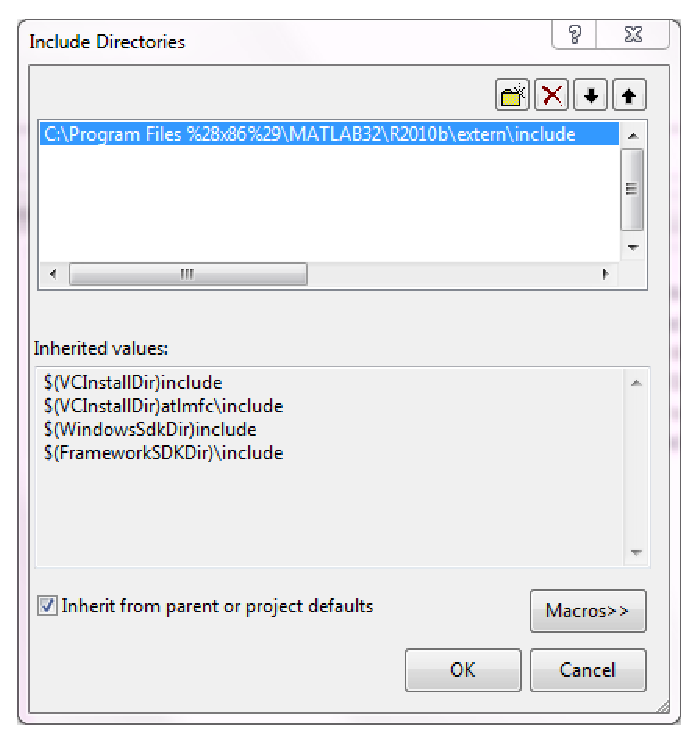
\includegraphics[scale = 0.6]{SettingIncludeFolder.eps}
\caption{MATLAB Include Settings}
\label{fig:SettingIncludeFolder}
\end{figure}


\begin{enumerate}
\item Open Visual C++
\item Select ``File | Open | Project/Solution...'' from the menu bar
\item Browse to the GmatDevelopment\textbackslash build\textbackslash GmatVS2010 folder
\item Select the GmatVS2010.sln solution file and click the Open button.  The GMAT solution will open and show projects to build GMAT and several plugin libraries.
\item Set your include and library paths for the libMatlabInterface and libFminconOptimizer projects.  This is done by following these steps for each project:
\begin{enumerate}
\item Right click on the project node (either libMatlabInterface or libFminconOptimizer)
\item Select the ``Properties'' entry on the pop-up menu
\item On the dialog that appears, set the Configuration to ``All Configurations''
\item Select the ``Configuration Properties | VC++ Directories'' entry on the property tree in the left panel of the dialog
\item Select the ``Include Directories'' line, and select \textless Edit...\textgreater from the drop-down button that sets the directory list
\item A new dialog appears that lists the include directory settings for at the project scope.  Click on the first entry in the list, and then click on the button to its right labeled with ellipses (...)
\item A file browser will appear.  Navigate in this browser to your MATLAB folder, and then inside of it, navigate to the ``extern\textbackslash include'' folder.  This folder contains the header files GMAT needs to build the interface.  Click the ``Select Folder'' button to select it.
\item Once the file browser window closes, your include dialog should resemble the one shown in Figure~\ref{fig:SettingIncludeFolder}.  Press the OK button.
\end{enumerate}
\item Right click on the libMatlabInterface project, and select Build.  (Don't select Rebuild unless you want to also rebuild libGmatBase.dll).
\item Right click on the libFminconOptimizer project, and select Build.  (Don't select Rebuild unless you want to also rebuild libGmatBase.dll and libMatlabInterface.dll).
\item Open a windows explorer and browse to your GmatDevelopment\textbackslash application\textbackslash bin folder.  You should see libMatlabInterface.dll and libFminconOptimizer.dll in the folder now.
\item Double click on the GMAT.exe file to run GMAT.  fmincon will now appear as an option in the Solvers | Optimizers entry of the resource tree.
\end{enumerate}

\section{\label{sec:Plugins}Standard GMAT Plugins}

There are three additional plugin libraries that are built for GMAT at this writing.  If you have access to the plugin repositories, you can configure and build these optional libraries: libDataFile, libCcsdsEphemerisFile, and libVF13Optimizer.  The VF13ad optimizer library, like the Estimation library described above, uses the Fortran to C library, so if you plan to build it, follow the steps above to setup either f2c or SPICE.  The DataFile plugin and the CcsdsEphemerisFile plugin use the C++ extensions to the Perl Compatible Regular Expression library, pcrecpp.  Configuration of that component is described next.

\subsection{Configuring and Building PCRECPP (Optional)}

GMAT uses the C++ version of the Perl Compatible, pcrecpp, for string manipulation when working with data files and CCSDS based ephemeris products.  The following steps describe how to set up pcrecpp.

\begin{enumerate}
\item Download the pcre 8.12 (to guarantee project file consistency -- preassembled Visual C++ 2010 solutions are packaged in the GMAT repository; other versions may require some modification to the build configuration) from ftp://ftp.csx.cam.ac.uk/pub/software/programming/pcre/
\item Unpack the download into your Gmat3rdParty/pcre folder.  This will give you a folder named pcre-\textless version\textgreater, where \textless version\textgreater is the version number for the library.  (For me, the resulting folder is Gmat3rdParty/pcre/pcre-8.12.)
\item Copy the contents of pcre-8.12 into the pcre folder, moving them up one level.  This places the header files in the location needed to build the plugins.
\item The usual way to build pcre is to download and install CMake for your platform, use it to create build files (Makefiles on unix like systems, project files and solution files on Windows), and then build from those files. The Windows pcre library files have already been created for pcre-8.12, and can be found in the GMAT plugins build folder build\textbackslash windows-VS2010 in the archive pcre-VS2010-out.zip.
\item Locate pcre-VS2010-out.zip.
\item Unpack its contents into your pcre folder.  This will create a lib and a dll folder in your pcre folder.
\item Copy the contents of the pcre\textbackslash dll folder into your GMAT executable folder.
\end{enumerate}

This completes the pcre setup.  If you'd prefer to compile pcre yourself, the instructions for doing this using CMake can be found in the pcre\textbackslash NON-UNIX-USE file.  Just be sure that you place the resulting libraries in place in pcre\textbackslash lib and pcre\textbackslash dll.

\subsection{Building the DataFile, CCSDS Ephemeris File, and VF13ad Plugins}

\textit{Instructions to be written as needed}

\begin{thebibliography}{9}
\bibitem {VisualStudio} Visual Studio Express can be downloaded from http://www.microsoft.com/express/Downloads/\#2010-Visual-CPP

\bibitem {wx} http://wxwidgets.org/downloads/

\bibitem {spice} http://naif.jpl.nasa.gov/naif/index.html

\end{thebibliography}


\appendix

\section{\label{sec:DataFileLayout}GMAT Data Files and Support Files }

GMAT requires access to data files organized in a file structure described in the GMAT startup file, gmat\_startup\_file.txt.  That file should be in the folder from which GMAT is launched.  In a typical setup, the GMAT startup file identifies a root folder, a data file folder, and then uses these two locations to identify the locations of additional data files needed by GMAT.  A typical startup file contains these lines for the top level folders:

\begin{quote}
\begin{verbatim}
ROOT_PATH              = ../
DATA_PATH              = ROOT_PATH/data/
\end{verbatim}
\end{quote}

\noindent The remaining lines in the file describe the locations of planetary ephemerides, coefficient files for planetary gravity fields, time system data, and other data elements needed when GMAT runs.  A typical file structure for the data files is shown in Figure~\ref{fig:DataFileStrucure}.  This file structure matches the structure delivered with GMAT R2011a.  It also matches the data file structure found in the source code repository for GMAT at SourceForge at the time of this writing.  The entries in the GMAT startup file point to specific files in this structure.  For example, the lines


\begin{figure}[htb]
  \begin{center}
	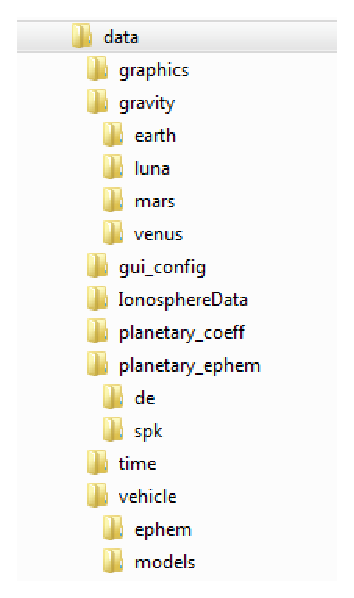
\includegraphics{DataFileLayout.eps}
	\caption{The Default Data File Strucure for GMAT}
	\label{fig:DataFileStrucure}
  \end{center}
\end{figure}


\begin{quote}
\begin{verbatim}
SPK_PATH               = DATA_PATH/planetary_ephem/spk/
PLANETARY_SPK_FILE     = SPK_PATH/de421.bsp
\end{verbatim}
\end{quote}

\noindent identify the location of the SPICE planetary ephemeris file, de421.bsp, in the file system.  Using the default entries provided thus far, GMAT looks for the file

\begin{quote}
\begin{verbatim}
../data/planetary_ephem/spk/de421.bsp
\end{verbatim}
\end{quote}

\noindent relative to the starting folder for the system.  The startup file provides similar path data for all of GMAT's data files; interested users should look in this file when trying to understand the data used when running a mission.

\section{\label{sec:ThirdPartyVersions}Library Versions}

At this writing, the software used to populate the Gmat3rdParty folder is as follows:

\begin{itemize}
\item wxWidgets,	2.8.12
\item The SPICE Toolkit, N0064
\item MATLAB, R2011a
\item pcre, 8.12
\item f2c, built from source last updated Sep 3, 2010
\end{itemize}

\noindent These versions are the target versions for GMAT R2011b.

\section{\label{app:64bit}Building GMAT in 64-bit mode}

\textit{To be written as needed}

\end{document}
